% Capítulo 9: árvore de chamadas da recursão ingênua de fib(5), com os subproblemas repetidos.
\documentclass[border=4pt]{standalone}
\usepackage[utf8]{inputenc}
\usepackage[T1]{fontenc}
% Estilo comum das figuras de árvores (capítulo 5).
\usepackage{tikz}
\usetikzlibrary{arrows.meta, positioning, calc}
\definecolor{navy}{RGB}{23,45,80}
\definecolor{laranja}{RGB}{250,110,29}
\definecolor{cinzalogo}{RGB}{107,114,126}
\tikzset{
  vertice/.style={circle, draw=navy, line width=0.9pt, fill=laranja!12, minimum size=8mm,
                  inner sep=0pt, font=\sffamily\small},
  destaque/.style={vertice, fill=laranja!45, draw=laranja},
  apagado/.style={vertice, dashed, draw=cinzalogo, fill=white, text=cinzalogo},
  arvore/.style={level distance=12mm, edge from parent/.style={draw=navy, line width=0.9pt}},
  rotulo/.style={font=\sffamily\small\bfseries, text=navy},
  legenda/.style={font=\sffamily\scriptsize, text=cinzalogo},
  setanova/.style={-{Stealth[length=2.2mm]}, laranja, line width=1.3pt},
}

\tikzset{
  chamada/.style={rectangle, rounded corners=2pt, draw=navy, line width=0.8pt, fill=white,
                  minimum width=9mm, minimum height=6mm, inner sep=1pt, font=\sffamily\small},
  rep3/.style={chamada, fill=laranja!45, draw=laranja},
  rep2/.style={chamada, fill=laranja!15},
  level 1/.style={sibling distance=56mm},
  level 2/.style={sibling distance=26mm},
  level 3/.style={sibling distance=13mm},
  level 4/.style={sibling distance=11mm},
}
\begin{document}
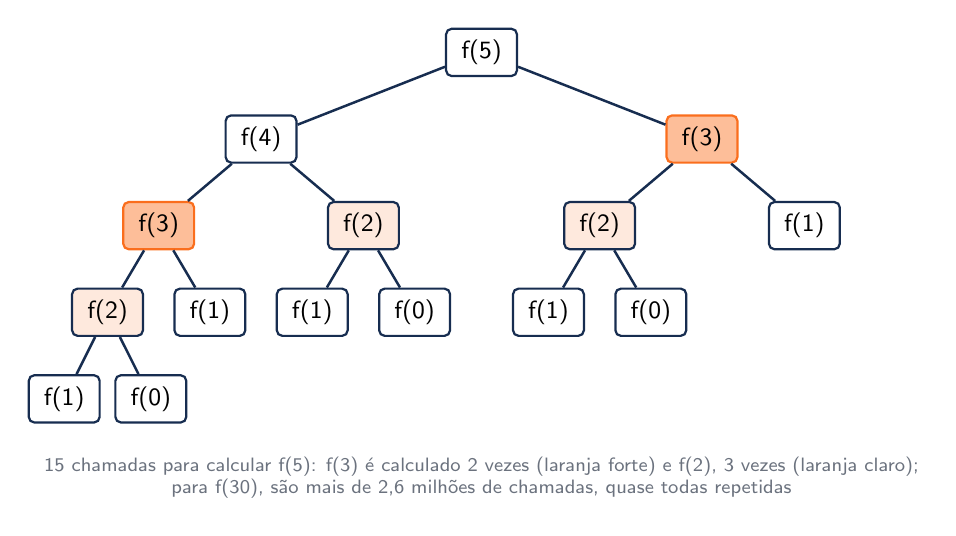
\begin{tikzpicture}[arvore, level distance=11mm]
  \node[chamada] {f(5)}
    child { node[chamada] {f(4)}
      child { node[rep3] {f(3)}
        child { node[rep2] {f(2)}
          child { node[chamada] {f(1)} }
          child { node[chamada] {f(0)} } }
        child { node[chamada] {f(1)} } }
      child { node[rep2] {f(2)}
        child { node[chamada] {f(1)} }
        child { node[chamada] {f(0)} } } }
    child { node[rep3] {f(3)}
      child { node[rep2] {f(2)}
        child { node[chamada] {f(1)} }
        child { node[chamada] {f(0)} } }
      child { node[chamada] {f(1)} } };
  \node[legenda, align=center] at (0, -5.4)
    {15 chamadas para calcular f(5): f(3) é calculado 2 vezes (laranja forte) e f(2), 3 vezes (laranja claro);\\
     para f(30), são mais de 2,6 milhões de chamadas, quase todas repetidas};
\end{tikzpicture}
\end{document}
